\documentclass[runningheads,a4paper]{llncs}

\usepackage{amssymb}
\setcounter{tocdepth}{3}
\usepackage{graphicx}

\usepackage{url}
\newcommand{\keywords}[1]{\par\addvspace\baselineskip
\noindent\keywordname\enspace\ignorespaces#1}

% Additional packages
\usepackage[utf8]{inputenc}
\usepackage{tikz}

% TiKZ styles
\tikzstyle{var} = [circle,
                   thick,
                   draw, fill=red!20,
                   text width=4.5em,
                   text badly centered,
                   node distance=3cm,
                   inner sep=0pt]

\tikzstyle{factor} = [rectangle,
                      thick,
                      draw, fill=blue!20,
                      text width=1em,
                      text centered,
                      minimum height=3em,
                      minimum width=3em]

\tikzstyle{line} = [draw]

\begin{document}

\mainmatter  % start of an individual contribution

% first the title is needed
\title{Semantic Novelty Detection with Graphical Models
on Dora Architecture}

% a short form should be given in case it is too long for the running head
% \titlerunning{Lecture Notes in Computer Science: Authors' Instructions}

% the name(s) of the author(s) follow(s) next
%
% NB: Chinese authors should write their first names(s) in front of
% their surnames. This ensures that the names appear correctly in
% the running heads and the author index.
%
\author{André Susano Pinto}
%
%\authorrunning{Lecture Notes in Computer Science: Authors' Instructions}
% (feature abused for this document to repeat the title also on left hand pages)

% the affiliations are given next; don't give your e-mail address
% unless you accept that it will be published
\institute{Faculdade de Engenharia da Universidade do Porto, Portugal\\
\url{andresusanopinto@gmail.com}\\
\url{http://url}}

\toctitle{Lecture Notes in Computer Science}
\tocauthor{Authors' Instructions}
\maketitle


\begin{abstract}
This papers presents an approach on implementing novelty detection at semantic level
for indoor room classification in Dora. \emph{Graphical models} are used to model
probabilistic knowledge and novelty detection is implemented on top of them.
The novelty threshold is then optimized using an unconditional probability density
model that is trained from unlabelled data.

\keywords{novelty detection, semantic data, graphical models, room classification,
indoor environments, robotics.}
\end{abstract}


%%%%%%%%%%%%%%%%%%%%%%%%%%%%%%%%%%%%%%%%%%%%%%%%%%%%%%%%%%%%%%%%%%%%%%
\section{Introduction}
\begin{itemize}
\item Explain context of indoor room categorization and importance of novelty detection.
\end{itemize}

There has been several efforts in the area of Artificial Intelligence and Robotics in creating robots
that are able to interact with humans and their environments.
One of the existing problems is a reliable high-level localization method that can be deployed into new
and unknown environments.
In this article we focus on the mapping, using \emph{semantic data}, of indoor environments such as houses and offices to room categories
such as kitchen, corridor, office.
And how to perform novelty detection on them: \emph{detect a new room category that was not present in the labelled data}.

Dora\cite{dora} (CogX: Dora) was used as a base system where this novelty detection would be implemented.
As Dora moves through the environment its \emph{conceptual layer} builds a structural and probabilistic representation of the space
instantiated as a \emph{graphical model}.
That model connects the sensed properties together with the variables used to model the world.
And allows to perform queries on the probabilities of aspects of the environment.
For example: where is the robot most likely to find a cereal box\cite{exploiting}.

\subsection{Semantic Data}
\begin{itemize}
\item Explain what we mean by semantic data and how its captured by Dora
\end{itemize}

Dora has a set of machine learning tools that are used to sense the environment around it.
The output of those describe a certain high-level property or information that we refer as \emph{semantic data}.
The following types of probabilistic information are extracted by Dora and used on this paper:
\begin{description}
\item[Object detection] is performed by running several pre-trained object detectors on the visual input. The system becomes
aware of the presence of objects such as book, cereal box, computer, robot, stapler, toilet paper.

\item[Room Size and Shape] are extracted by using the 2D laser scans. The system categorizes each room in terms of its size (large, medium, small) and shape (rectangular and elongated).

\item[Room Appearance] is categorized using CRFH and a pre-trained set of 7 different models.

\item[Doorway detection] is used to segment the low-level space into rooms and map connectivity between them.
\end{description}

\subsection{Graphical Models}
\begin{itemize}
\item Explain Dora use of Graphical Models
\end{itemize}

Dora uses \emph{chain graphs} as modelling tool. Those can be converted to \emph{factor graphs}\cite{factor}.

\begin{figure}[h]
\centering
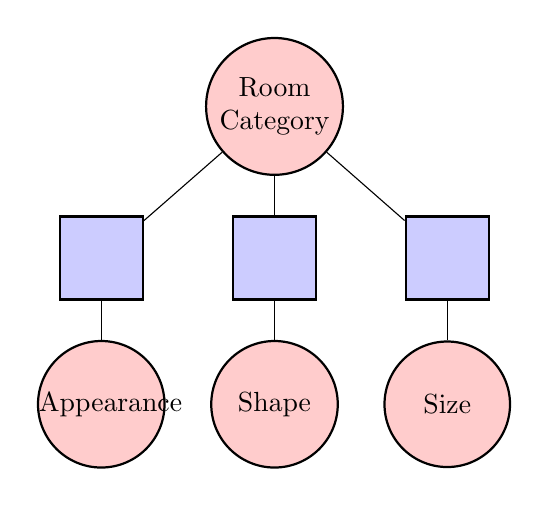
\begin{tikzpicture}[node distance = 2cm, auto]
    \matrix[row sep=0.5cm,column sep=0.5cm] {
      & \node [var] (room) {Room Category}; \\
      \node [factor] (fAppearance) {}; &
      \node [factor] (fShape) {}; &
      \node [factor] (fSize) {}; \\

      \node [var] (appearance) {Appearance}; &
      \node [var] (shape) {Shape}; &
      \node [var] (size) {Size}; \\
    };
  \path [line] (room) -- (fAppearance);
  \path [line] (room) -- (fShape);
  \path [line] (room) -- (fSize);

  \path [line] (fAppearance) -- (appearance);
  \path [line] (fShape) -- (shape);
  \path [line] (fSize) -- (size);
\end{tikzpicture}
\caption{Example of a factor graph used for Dora for representing the environment.}
\end{figure}

%%%%%%%%%%%%%%%%%%%%%%%%%%%%%%%%%%%%%%%%%%%%%%%%%%%%%%%%%%%%%%%%%%%%%%
\section{Novelty Detection}
\begin{itemize}
\item Explain 
\item Approach with a threshold function
\item Need of a normalizing factor for a threshold with dynamic functions
\item Usage of conditional density
\item Assuming of every output is equally likely
\item Using unlabelled data
\end{itemize}

Novelty detection can be performed by a threshold function sorting the input space in an optimal way to
decrease error in detection.

Its harder than a classification problem as the system only has access to positive samples.
Under that a common approach is to use conditional probability $P(x|known)$ as a threshold.

\subsection{Stable threshold}
Although in our case we are dealing with a dynamic graph $G$ that keeps changing through time as new variables
are added. Which increases the dimension of our space and spreads the distribution over the variables.

This turns it impossible to directly train a threshold function on $P_G(x)$, as we cannot assume $P(x)$ to be constant over any set of $x$.
So we need to describe $P(x)$ to develop a stable threshold on $P_G(x)/P(x)$.

A common assumption is that every possible input is equally likely then the threshold
should be $P_G(x)/(\prod |x_i|)$.

\subsection{Unlabelled data}
Nonetheless in the case of robotics its often the case we can access large amounts of unlabelled data.
This leads to an interesting point that instead of assuming a constant $P(x)$ we can actually try to build
model for it.

Under that we decided to test assuming that all probabilities are independent. That can be modelled as a graph $G'$.
And corresponding function $P_G(x)/P_{G'}(x)$.

This way our unconditional function perceive which features are slightly more biased to a certain value and will
compensate on the probability calculation.

This step is important to achieve a correct order of the input space.


%%%%%%%%%%%%%%%%%%%%%%%%%%%%%%%%%%%%%%%%%%%%%%%%%%%%%%%%%%%%%%%%%%%%%%
\section{Results}
\begin{itemize}
\item Show results and how much it improves by using a simple method for unconditional probability
\end{itemize}

%%%%%%%%%%%%%%%%%%%%%%%%%%%%%%%%%%%%%%%%%%%%%%%%%%%%%%%%%%%%%%%%%%%%%%
\section{Conclusions and Future Work}
\begin{itemize}
\item Show a correct estimation of unconditional probability to be important in estabilishing a novelty detection threshold
\item Show unlabelled data can be used for it.
\item Although focus on Room Categorization we expect the results and techniques to be usable on other areas.
\end{itemize}

%%%%%%%%%%%%%%%%%%%%%%%%%%%%%%%%%%%%%%%%%%%%%%%%%%%%%%%%%%%%%%%%%%%%%%
\begin{thebibliography}{4}

\bibitem{jour} Smith, T.F., Waterman, M.S.: Identification of Common Molecular
Subsequences. J. Mol. Biol. 147, 195--197 (1981)

\bibitem{lncschap} May, P., Ehrlich, H.C., Steinke, T.: ZIB Structure Prediction Pipeline:
Composing a Complex Biological Workflow through Web Services. In: Nagel,
W.E., Walter, W.V., Lehner, W. (eds.) Euro-Par 2006. LNCS, vol. 4128,
pp. 1148--1158. Springer, Heidelberg (2006)

\bibitem{book} Foster, I., Kesselman, C.: The Grid: Blueprint for a New Computing
Infrastructure. Morgan Kaufmann, San Francisco (1999)

\bibitem{proceeding1} Czajkowski, K., Fitzgerald, S., Foster, I., Kesselman, C.: Grid
Information Services for Distributed Resource Sharing. In: 10th IEEE
International Symposium on High Performance Distributed Computing, pp.
181--184. IEEE Press, New York (2001)

\bibitem{proceeding2} Foster, I., Kesselman, C., Nick, J., Tuecke, S.: The Physiology of the
Grid: an Open Grid Services Architecture for Distributed Systems
Integration. Technical report, Global Grid Forum (2002)

\bibitem{url} National Center for Biotechnology Information, \url{http://www.ncbi.nlm.nih.gov}

\end{thebibliography}

\end{document}
